% figures/infinite-paths.tex

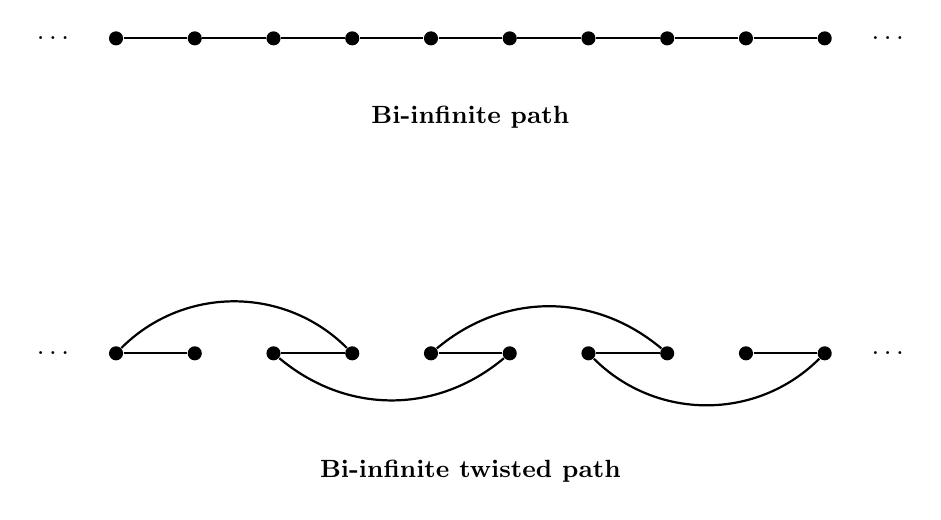
\begin{tikzpicture}[
    vertex/.style={circle, fill, inner sep=1.8pt},
    edge/.style={thick},
    caption/.style={font=\small\bfseries, node distance=1.5cm}
]

    % --- Subfigure 1: Bi-infinite Path (Top) ---
    \begin{scope}[yshift=4cm]
        % Vertices -4 to 5
        \foreach \x in {-4,...,5}
            \node[vertex] (v\x) at (\x, 0) {};
            
        % Consecutive horizontal edges
        \foreach \x [evaluate=\x as \nextx using int(\x+1)] in {-4,...,4}
            \draw[edge] (v\x) -- (v\nextx);
            
        % Continuation dots
        \node at (-4.8, 0) {$\dots$};
        \node at (5.8, 0) {$\dots$};
        
        % Caption for the first graph
        \node[caption] at (0.5, -1) {Bi-infinite path};
    \end{scope}

    % --- Subfigure 2: Matching and Arcs (Bottom) ---
    \begin{scope}[yshift=0cm]
        % Vertices -4 to 5
        \foreach \x in {-4,...,5}
            \node[vertex] (u\x) at (\x, 0) {};
            
        % Specified horizontal edges (the matching)
        \foreach \a/\b in {-4/-3, -2/-1, 0/1, 2/3, 4/5}
            \draw[edge] (u\a) -- (u\b);
            
        % Upper arcs
        \draw[edge] (u-4) to[bend left=45] (u-1);
        \draw[edge] (u0) to[bend left=40] (u3);
        
        % Lower arcs
        \draw[edge] (u-2) to[bend right=40] (u1);
        \draw[edge] (u2) to[bend right=45] (u5);

        % Continuation dots
        \node at (-4.8, 0) {$\dots$};
        \node at (5.8, 0) {$\dots$};
        
        % Caption for the second graph
        \node[caption] at (0.5, -1.5) {Bi-infinite twisted path};
    \end{scope}

\end{tikzpicture}